\documentclass[a4paper]{article}
\usepackage[utf8]{inputenc}
\usepackage[spanish, es-tabla]{babel}

\usepackage{amsmath}
\usepackage{amsfonts}
\usepackage{amssymb}

\usepackage{float}
\usepackage{graphicx}
\graphicspath{ {./Imagenes/} }

\usepackage[american voltages,american currents]{circuitikz}

\usepackage{fancyhdr}

\usepackage{units} 

\pagestyle{fancy}
\fancyhf{}
%\lhead{23.09 Física Electrónica}
\rhead{Bertachini, Lambertucci, Londero, Mechoulam, Musich}
\rfoot{Página \thepage}


\begin{document}

%%%%%%%%%%%%%%%%%%%%%%%%%%%%%%%%%%%%%%%%%%%%%%%%%%%%%%%%%%%%%%%%%%%%%%%%% 
%								CARATULA								%
%%%%%%%%%%%%%%%%%%%%%%%%%%%%%%%%%%%%%%%%%%%%%%%%%%%%%%%%%%%%%%%%%%%%%%%%% 

\begin{titlepage}
\newcommand{\HRule}{\rule{\linewidth}{0.5mm}}
\center
\mbox{\textsc{\LARGE \bfseries {Instituto Tecnológico de Buenos Aires}}}\\[1.5cm]
\textsc{\Large 23.09 Física Electrónica}\\[0.5cm]

\HRule \\[0.6cm]
{ \Huge \bfseries Trabajo práctico N$^{\circ}$1}\\[0.4cm] 
\HRule \\[1.5cm]


{\large

\emph{Grupo 5}\\
\vspace{3px}

\begin{tabular}{lr}
\textsc{Bertachini}, Germán  & 58750 \\ 	
\textsc{Lambertucci}, Guido Erinque  & 58009 \\
\textsc{Londero Bonaparte}, Tomás Guillermo  & 58150 \\
\textsc{Mechoulam}, Alan  &  58438\\
\textsc{Musich}, Francisco  & 58124 \\

\end{tabular}

\vspace{20px}

\emph{Profesores}\\
\vspace{3px}
\textsc{Baez}, Eduardo Diocles\\ 	
\textsc{Cesaretti}, Juan Manuel\\ 
\textsc{Douthat}, Analia Elizabeth\\ 
\textsc{Gardella}, Pablo Jesús\\ 	

\vspace{100px}

\begin{tabular}{ll}

Presentado: & 24/06/19\\

\end{tabular}

}

\vfill

\end{titlepage}


%%%%%%%%%%%%%%%%%%%%%%%%%%%%%%%%%%%%%%%%%%%%%%%%%%%%%%%%%%%%%%%%%%%%%%%%% 
%								INFORME									%
%%%%%%%%%%%%%%%%%%%%%%%%%%%%%%%%%%%%%%%%%%%%%%%%%%%%%%%%%%%%%%%%%%%%%%%%%

\section*{Introducción}

En el trabajo presente se llevó adelante el estudio de distintos tipos de diodos y circuitos, con el objetivo de llevar a la práctica la teoría estudiada en clases.

\section*{Desarrollo de la experiencia}

Primero se analizaron tres diodos distintos: rectificador 1N4148, zener y LED rojo, conectados de la forma presentada en el circuito (\ref{circ:1}).

\begin{figure}[H]
\begin{center}
\begin{circuitikz}
\draw
	(4,0)	to (0,0)
	(0,1.5)	to [sV,v_=$V$]	(0,0)
	(0,1.5)	to [R, l_=$ 470 \ \Omega $]	(4,1.5)
	(4,0)	to [Do, l_=Diodo analizado]	(4,1.5)
;\end{circuitikz}
\end{center}
\caption{Circuito utilizado para medir los diodos.}
\label{circ:1}
\end{figure}

Utilizando multimetros se observó el comportamiento de estos para ciertas tensiones y posteriormente se graficaron las curvas correspondiente a cada uno.

\begin{figure}[H]
	\centering
	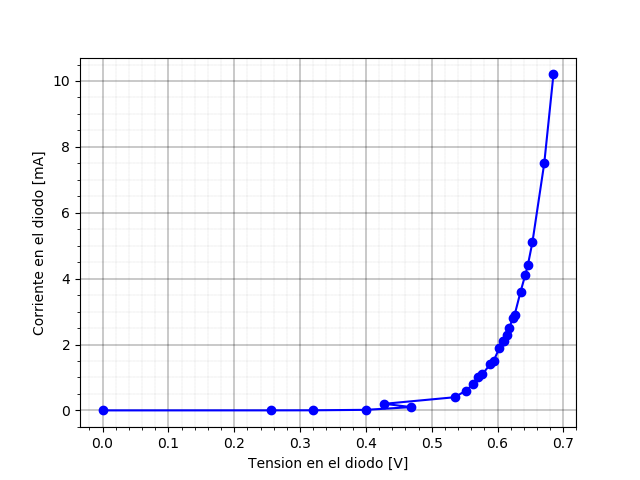
\includegraphics[width=0.8\textwidth]{CurvaDiodoRectificador.png}
	\caption{Corriente en función de la tensión del diodo rectificador 1N4148.}
	\label{fig:diodorect}
\end{figure}

\begin{figure}[H]
	\centering
	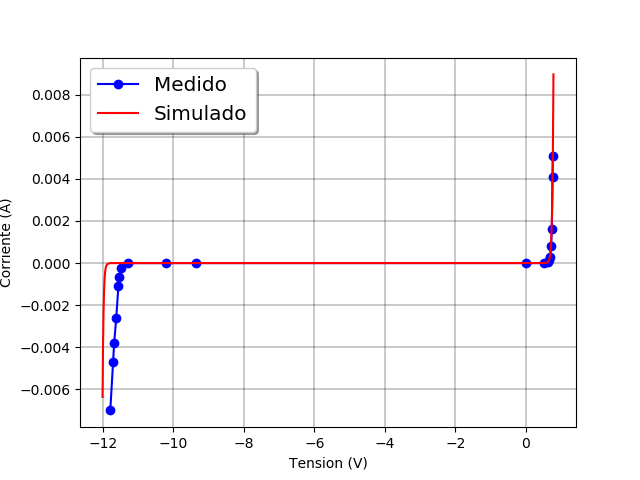
\includegraphics[width=0.8\textwidth]{CurvaZenerEntera.png}
	\caption{Corriente en función de la tensión del diodo zener.}
	\label{fig:diodozen}
\end{figure}

\begin{figure}[H]
	\centering
	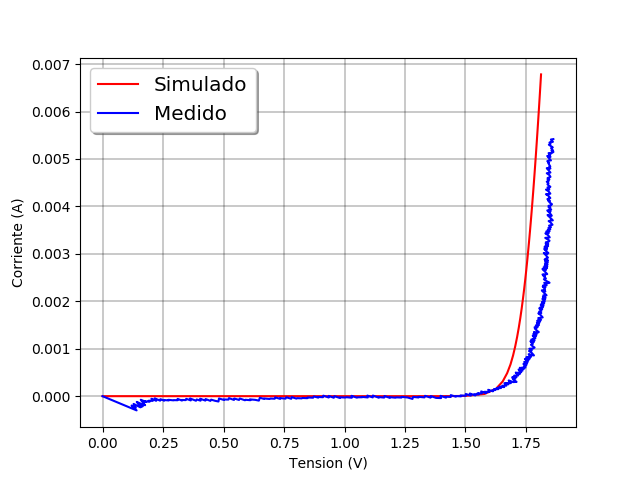
\includegraphics[width=0.8\textwidth]{CurvaDiodosLed.png}
	\caption{Corriente en función de la tensión del diodo LED.}
	\label{fig:diodoled}
\end{figure}




Luego se simuló el circuito brindado por la cátedra.
\begin{figure}[H]
	\centering
	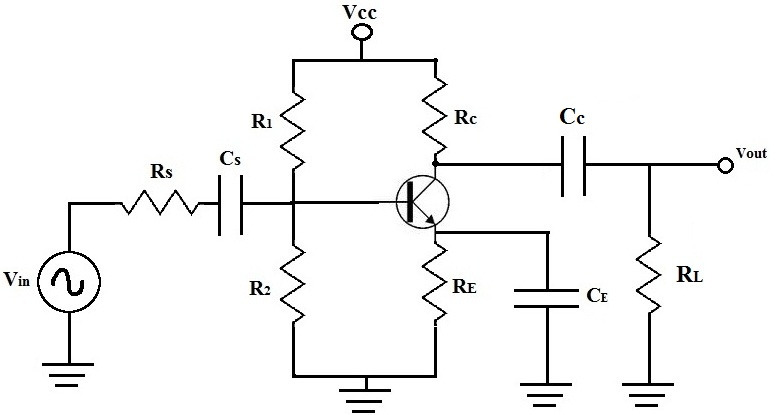
\includegraphics[width=0.5\textwidth]{commonEmitter.jpg}	
	\caption{Circuito provisto por la catedra.}
	\label{fig:cmnemitnpn}

\end{figure}
Analizando la función transferencia de tensión de este, se observa que la transferencia para la zona constante es de $44,36 \ dB$, siendo de $43,19 \ dB$ el valor obtenido en simulación.

\begin{figure}[H]
	\centering
	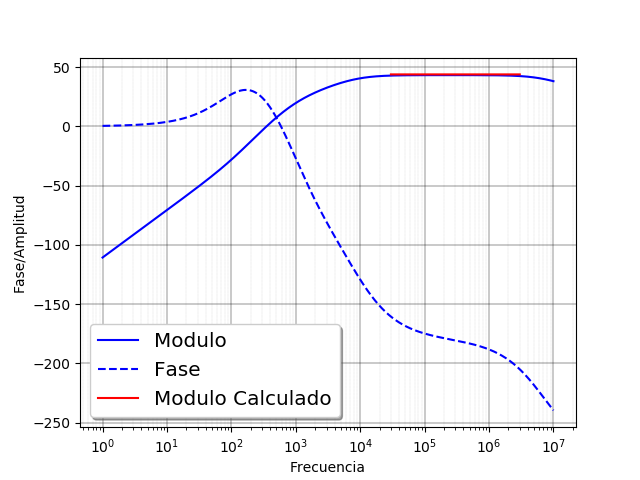
\includegraphics[width=0.8\textwidth]{RtaF2.png}	
	\caption{Diagrama de BODE para el cirucito dado.}
	\label{fig:bode}
\end{figure}

Finalmente se analizó la respuesta en frecuencia del circuito (\ref{circ:3}).

\begin{figure}[H]
\begin{center}
\begin{circuitikz}
\draw

	(0,0)	to (4,0)
	(0,1.5)	to [sV,v_=$AC$]	(0,0)
	(0,2.5)	to [V,v_=$DC$]	(0,1.5)
	(0,2.5)	to[R,l=$R_G$,a=$50\Omega$] (2,2.5)
	(0,2.5)	to[R,l=$R_G$] (2,2.5)
	(2,2.5)	to[R,l=$R$,a=$0.5M\Omega$] 	(4,2.5)
	(2,2.5)	to[R,l=$R$] 	(4,2.5)
	(4,0)	to [Do, l_=D1N4007]	(4,2.5)
;\end{circuitikz}
\end{center}
\caption{Circuito utilizado para medir los diodos.}
\label{circ:3}
\end{figure}

\begin{figure}[H]
	\centering
	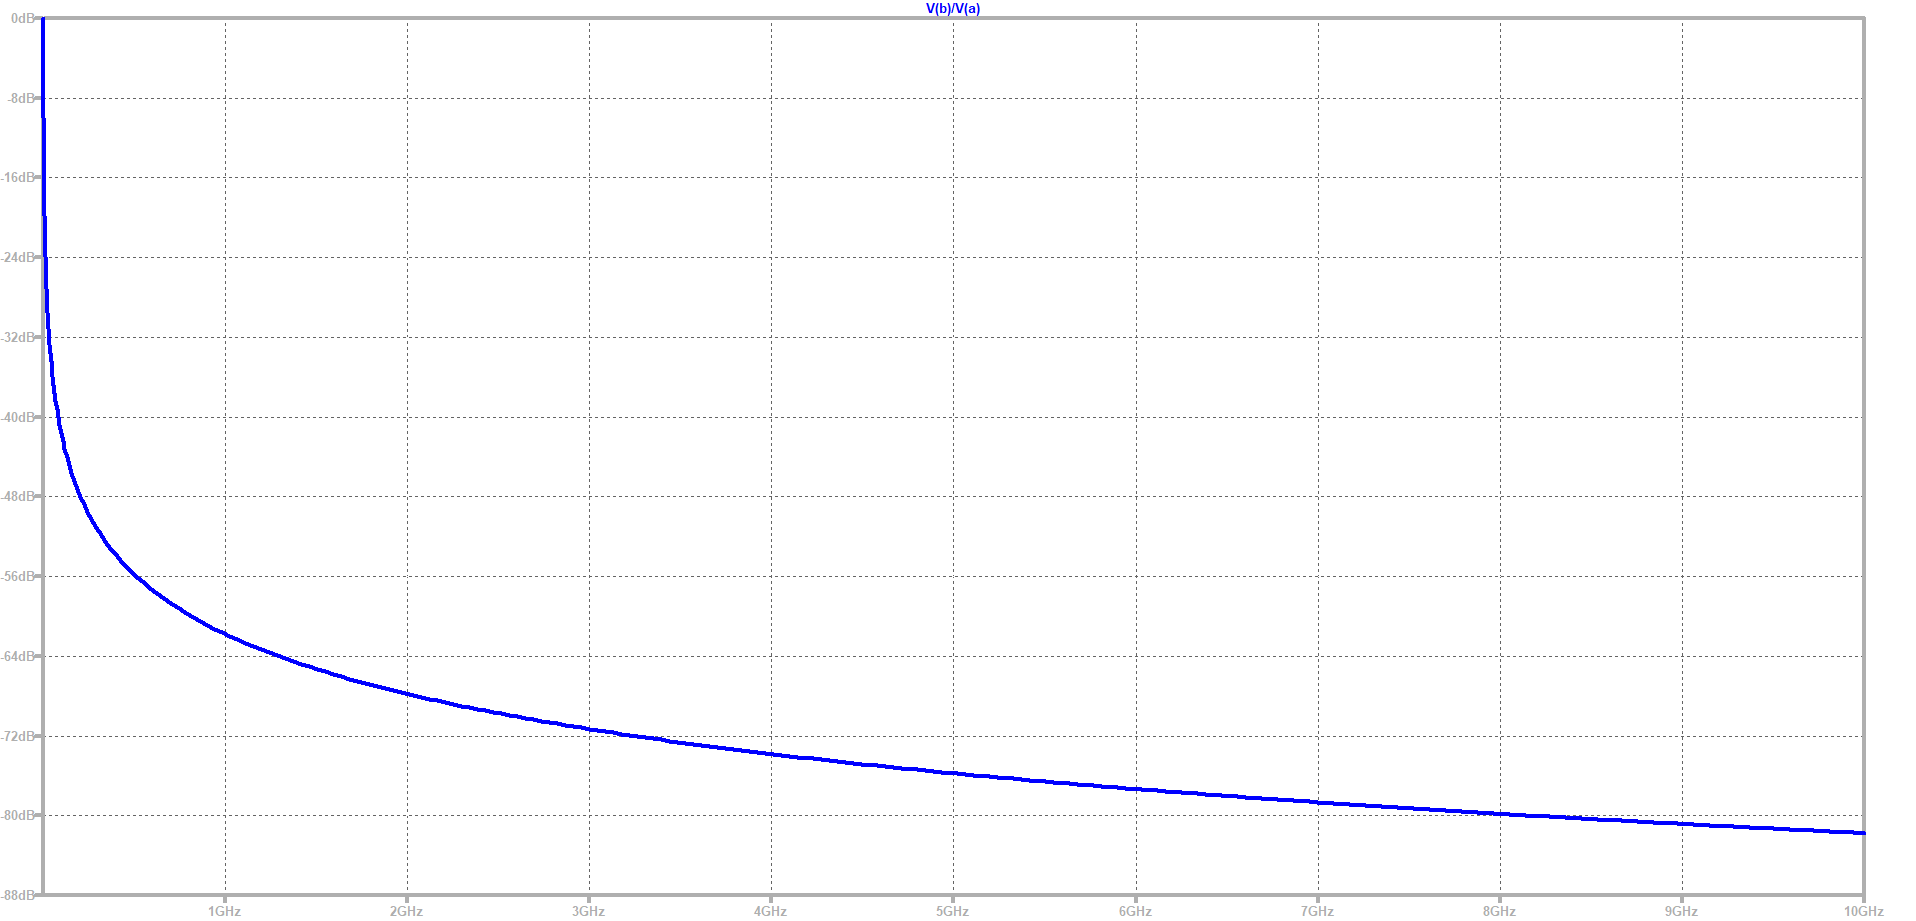
\includegraphics[width=0.8\textwidth]{RtaF3.png}	
	\caption{Respuesta en frecuencia del diodo D1N4007.}
	\label{fig:rtaf}
\end{figure}
Como se puede observar en el gráfico, estamos en presencia de un filtro pasabajos con una frecuencia de corte estimada de 165KHz. Se podría decir que presenta aproximadamente un cero en $1 \ Hz$ y un polo en $8 \ KHz$, ambos de orden 1.
El comportamiento del diodo se asocia con el de un capacitor, el valor equivalente de dicho capacitor será calculado como:
\begin{center}
$c=\dfrac{1}{2\pi Rf}$
\end{center}
Los valores obtenidos fueron los siguientes:
\begin{center}
$C= 1,93 pF$
\end{center}

\begin{figure}[H]
\begin{center}\begin{circuitikz}[scale=1.6]\draw
(0,1) to[V, l=$DC$,a=$5V$] (0,2)
(0,0) to[sV, l=$AC$,a=$1V$] (0,1)
(0,2) to[R,l=$R_G$]  (2,2)
(2,2) -- (4,2)
(2,2) to[R,l=$R_D$,a=$0.5M\Omega$] (2,0)
(4,0)	to [C, l=$C$,a=1.93pF]	(4,2)
(0,0) -- (4,0);
\end{circuitikz} 
\caption{Circuito equivalente del diodo}
\end{center}
\end{figure}

El fabricante en su hoja de datos declara una capacitancia de juntura típica de $15 pF$.

\section*{Conclusión}

Los resultados obtenidos al estudiar los tres primeros diodos se corresponden con los resultados esperados. Se observan pequeñas incongruencias en los gráficos, como por ejemplo en el gráfico (\ref{fig:diodorect}), que son atribuidos a cambios de escala de los instrumentos durante el análisis.\newline
Luego se comprobó que, la función transferencia del segundo análisis, es acorde a la real, dejando pasar las frecuencias altas, acorde a lo esperado.\newline
Por último, la respuesta en frecuencia del último punto mostró que un diodo conectado de esa forma se puede asociar a un capacitor. Esto se sustenta en que la capacitancia declarada por el fabricante es similar a la obtenida mediante un proceso de simulación.


\end{document}

